\chapter{Stato dell'arte}

\section{Studi sull’engagement all’interno degli ambienti di studio}
Gli studi ritrovati che effettuano quest’analisi o trattano un argomento simile sono:
\subsection{Riconoscimento delle emozioni cognitive in ambiente di e-learning}
In questo studio (\cite{RecoCognEmoELearnEnv}) gli stati di d’animo che vengono classificati dal loro sistema sono i seguenti:
\begin{itemize}
    \item Entusiasmo,
    \item Interesse,
    \item Sorpresa,
    \item Noia,
    \item Perplessità,
    \item Frustrazione,
    \item Neutrale
\end{itemize}

Viene riportato che gli stati d’animo positivi (entusiasmo, interesse e sorpresa) sono spesso associati al raggiungimento del “flow state” da parte dello studente.

Più il singolo soggetto mantiene costante un mood positivo, tanto più permarrà in questo flow state, con esito un apprendimento più veloce ed efficace \cite{RecoCognEmoELearnEnv}.

Il raggiungimento di questo mood è stato inoltre connesso alla capacità dei singoli studenti di percepirsi come autosufficienti nel corso dell’attività di studio.

Questa percezione di sé stessi deriva dall’attitudine dello studente nel riuscire ad essere in controllo della sua personale situazione di studio, rispecchiandosi nella sua abilità di:
\begin{itemize}
    \item pianificare,
    \item controllare,
    \item dirigere
\end{itemize}
l’attività di apprendimento \cite{RecoCognEmoELearnEnv}.

È quindi necessario che gli studenti maturino una certa dimestichezza nello studio, e che vengano dunque supportati in vista dell’approccio ai problemi che vengono da loro riconosciuti in quanto difficili.

Naturalmente un sistema che permette di “leggere” con precisione lo stato d’animo di uno studente/studentessa o persino di un’intera classe, e quindi capire se questi si trovino nello stato di flow che possa permettere una migliore performance, è uno strumento utile per qualsiasi insegnante.

Un esempio circoscritto all’ambiente di lavoro potrebbe invece essere un’analisi del lavoratore nello svolgimento di un task e la possibilità, da parte di un capo progetto o di un tutor, di poter intervenire esclusivamente nel momento in cui il suo subordinato stia riscontrando dei problemi; in tal modo è permessa al dipendente una crescita professionale adeguata e non seguita al 100\%, così da sfruttare al meglio l’impiego del tempo del tutor.

\subsection {Le faccie dell'Engagement: Riconoscimento automatico dell'engagement degli studenti attraverso le espressioni facciali}

In \cite{FacesOfEngagement}, gli stati d’animo organizzati in scala da meno attento/a a più attento/a, sono:
\begin{itemize}
    \item Not engaged at all (Non coinvolto: che guarda da un’altra parte, che sta ovviamente non pensando al compito, occhi completamente chiusi)
    \item Nominally engaged (Formalmente coinvolto: occhi appena aperti, chiaramente non attento/a al task che sta svolgendo)
    \item Engaged in task (Coinvolto nel task: requisito che non richiede un’ammonizione per la progressione del task)
    \item Very engaged (Altamente coinvolto: lo/a studente/tessa potrebbe essere elogiato/a per il suo livello di coinvolgimento)
    \item Clip/frame non chiaro (l’immagine analizzata non contiene una persona o comunque non è possibile effettuare un’identificazione)
\end{itemize}

Lo studio si concentra sull’effettuare una stima dell’engagement degli studenti. 

È stato inizialmente sviluppato un metodo per rilevare automaticamente l’engagement, si è poi indagato su quali segnali siano utilizzati nel riconoscimento automatico effettuato dal computer per poi individuare quali strumenti vengano adoperati dagli insegnanti per risolvere il medesimo task.

Infine si è investigato sulla correlazione effettiva fra i risultati di queste analisi e la qualità delle performance degli studenti.

\begin{figure}
    \begin{center}    
        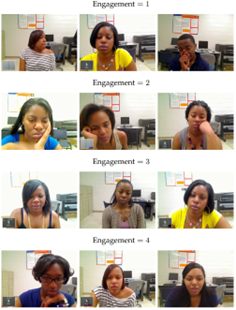
\includegraphics[width=0.4\linewidth]{images/2.png}
        \caption{Esempio campioni dal dataset dello studio}
    \end{center}
\end{figure}

\subsection{Codifica facciale come mezzo per il monitoraggio continuo del comportamento degli studenti nell'e-learning}

Il paper \cite{FacialCodingContinMonitor} si focalizza sul tracciamento continuo degli studenti, sia per quanto riguarda una vera e propria identificazione degli stessi attraverso il riconoscimento facciale, sia per calcolarne il livello di attenzione ed eventualmente stimarne le emozioni provate durante i corsi MOOCs (Massive Open Online Courses).

Per dirigere l’analisi del livello di attenzione, si è ricorso all’uso della libreria esterna Dlib, la quale consente di creare una mappatura delle caratteristiche facciali dello/a studente; per giunta, la piattaforma include anche un gaze tracker che lascia prevedere la direzione dello sguardo degli studenti durante lo svolgimento del corso.

Questi tre aspetti vengono successivamente congiunti al fine di creare un applicativo web per l’apprendimento, attraverso il quale, alla fine di ogni lezione, è possibile visionare in quale percentuale della durata del corso le persone hanno adempito alle metriche citate nell'immagine \ref{fig:image32}.

\begin{figure}
    \begin{center}    
        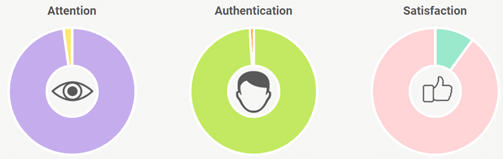
\includegraphics[width=1\linewidth]{images/3.png}
        \caption{Esempio di output del programma}
        \label{fig:image32}
    \end{center}
\end{figure}
 
\subsection{Predizione e localizzazione dell'engagement degli studenti in the wild}

Lo studio \cite{PredLocStudEngagInTheWild}, a differenza di altri, ha come premessa l’utilizzo delle immagini raccolte in ambienti non controllati per la creazione del modello che andrà successivamente ad effettuare la predizione per i nuovi campioni.

Per ambienti controllati, si intende setup di acquisizione dei video e delle immagini grazie ai quali non è possibile riscontrare problemi, quali scarsa illuminazione, occlusione ambientale, etc…

Per attuare ciò, sono stati sottoposti ad analisi molti studi precedentemente effettuati, per convenire al raccoglimento di campioni attraverso la fruizione, da parte dei soggetti, di video educazionali, categorizzando poi i vari video ed immagini ottenute in una scala, con valore da 0 a 3:
\begin{itemize}
    \item 0 \textrightarrow per niente interessato (il soggetto non sembra interessato e guarda spesso al di fuori dello schermo)
    \item 1 \textrightarrow poco interesse (il soggetto apre a malapena gli occhi, si muove in modo irrequieto sulla sedia)
    \item 2 \textrightarrow interessato/a al contenuto (sembra che al soggetto il contenuto riprodotto risulti interessante ed esso interagisce con questo)
    \item 3 \textrightarrow altamente interessato/a (il soggetto ha “gli occhi attaccati allo schermo” e risulta concentrato/a)
\end{itemize}


Hanno poi sfruttato un framework che esegue il riconoscimento dell’engagement e della localizzazione degli studenti.
\begin{itemize}
    \item Inizialmente vengono identificate la faccia e dei punti di riferimento all’interno di queste in ognuno dei frame analizzati 
    \item Procedendo, i video vengono suddivisi in segmenti più piccoli e le feature vengono estratte, “effettuando una media” dei risultati di ognuno dei frame.
    \item Si passa poi alla sequenza di frame successiva per effettuare la stessa analisi.
    \item Una volta raccolti tutti i dati, questi vengono elaborati per calcolarne l’engagement e la localizzazione attraverso la deep MIL network, impiegando la media e la top-k pooling per calcolarne la regressione.
\end{itemize}


\begin{figure}
    \begin{center}    
        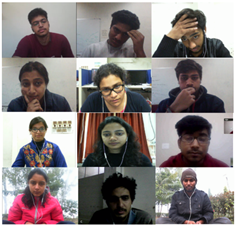
\includegraphics[width=0.8\linewidth]{images/4.png}
        \caption{Esempio di campioni dal dataset utilizzato in \cite{PredLocStudEngagInTheWild}}
    \end{center}
\end{figure}

\section{Cosa sono le AUs e il sistema FACS:}
FACS, acronimo di Facial Action Coding System, è un sistema di codifica delle espressioni facciali sviluppato dallo psicologo Paul Ekman e dal collega Wallace V. Friesen negli anni '70 \cite{PyFeat}.

Il sistema di codifica di FACS è composto da un insieme di codici numerici, o "Action Units" (AU), che rappresentano le azioni muscolari specifiche che avvengono durante le espressioni facciali. Ci sono 66 AUs, ciascuna delle quali rappresenta un'azione muscolare specifica, e ognuna di queste ha un codice numerico univoco.

La codifica delle FACS può essere utilizzata per identificare e descrivere le espressioni facciali in modo oggettivo e dettagliato. Ad esempio, un codificatore FACS identifica l'AU corrispondente al sollevamento di una delle due sopracciglia con codice 1, e l'AU corrispondente al sorriso con codice 12. 

Questi codici possono essere utilizzati per creare una descrizione dettagliata dell'espressione facciale di un individuo.

Le FACS sono state utilizzate in una vasta gamma di contesti, tra cui la ricerca scientifica, la valutazione clinica e la produzione di effetti speciali per il cinema e la televisione. 

Questo sistema è stato utilizzato con successo in molti contesti diversi ed è un metodo utile per descrivere le espressioni facciali in modo oggettivo e dettagliato. 

Sulla documentazione della libreria che ho utilizzato per l’estrazione delle AUs dal dataset aggregato ed utilizzato, è presente una tabella dove viene mostrato: il numero associato alla singola Action Unit, il loro relativo nome FACS, a quali muscoli della faccia sono correlate, la loro categoria FACS, le espressioni che vengono spesso legate a determinati valori di esse e i modelli che le utilizzano. Ho reso disponibile un estratto di questa \ref{Tab:Tabella_AUs} dove vengono presentate solo le Action Units utilizzate dalla libreria \cite{PyFeat} utilizzata per estrarre questi dati dalle immagini ma la tabella completa è consultabile sulla relativa pagina web.
\newpage
\begin{figure}
    \begin{center}    
        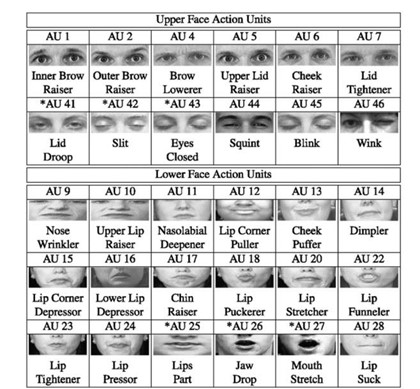
\includegraphics[width=1\linewidth]{images/10.jpg}
        \caption{Esempi di Action Units e le relativi sezioni facciali}
    \end{center}
\end{figure}

\section{Studi sul riconoscimento delle emozioni FACS per scelta del modello da utilizzare}
Essendo l’ammontare di studi che trattano l’analisi delle emozioni FACS maggiore rispetto a quelle che cercano di creare sistemi di riconoscimento automatico per gli stati d’animo, i quali possono direttamente aiutare a identificare i problemi nell’apprendimento delle conoscenze, ho ritenuto opportuno studiare e selezionare fra i modelli da questi proposti per l’elaborazione delle informazioni per il mio caso di studio.

Il paper con i migliori risultati che ho trovato è stato \cite{FaceExpreRecoImgSeqTwoFoldRandomForestClass}, in questo studio viene utilizzata una random forest a due livelli:
\begin{itemize}
    \item il primo livello è utilizzato per determinare le Action Units nelle sequenze di espressioni che vengono analizzate
    \item il secondo livello invece prende in input le Action Units estratte, ed effettua la classificazione delle espressioni finali
\end{itemize}

Il modello riesce ad ottenere una media di riconoscimento del 100\% per le Action Units e del 96.38\% per le espressioni facciali (emozioni) che risulta essere migliore degli studi successivamente riportati.

Prima ancora di arrivare al primo livello della random forest viene utilizzato il modello AAM che identifica i punti di riferimento sulla faccia del soggetto ripreso nel video analizzato (o nella sequenza di immagini analizzate) per poi ricorrere all’utilizzo del Lucas-Kanade optical flow tracker col fine di tracciare i punti di riferimento nei frame successivi.

Viene poi calcolato il vettore di spostamento fra i punti di riferimento trovati sul primo frame, dove il soggetto si presenta con un’espressione neutrale, e i punti di riferimento trovati nel frame finale dove l’espressione facciale è al suo picco espressivo. 
Questo vettore di spostamento viene utilizzato nel primo layer della random forest per l’estrazione delle Action Units.

Le espressioni facciali sono processi dinamici, conseguenza dell'attività muscolare di varie parti del volto:
\begin{itemize}
    \item fronte,
    \item occhi,
    \item naso,
    \item bocca,
    \item mascella,
    \item contorno
\end{itemize}

Le caratteristiche dinamiche possono essere rappresentate dalla differenza tra i vettori estratti dai fotogrammi. 

Le sei espressioni facciali di base:
\begin{itemize}
    \item felicità,
    \item tristezza,
    \item rabbia,
    \item disgusto,
    \item paura,
    \item sorpresa
\end{itemize}
possono essere descritte utilizzando le AUs, codificate in base ai coinvolgimenti muscolari facciali.

Il processo di estrazione delle caratteristiche di movimento di un’espressione facciale è illustrato nella figura \ref{fig:image1}.
\begin{figure}
    \begin{center}    
        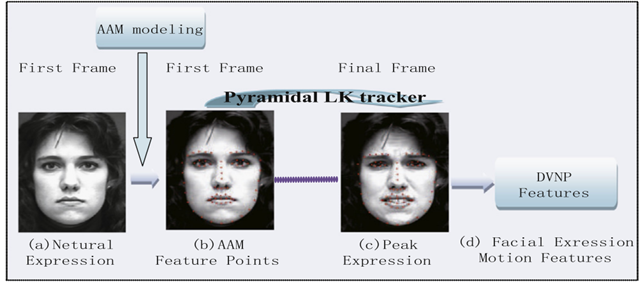
\includegraphics[width=1\linewidth]{images/14.png}
        \caption{Processo di estrazione dinamica delle feature delle espressioni facciali}
        \label{fig:image1}
    \end{center}
\end{figure}

Random Forest è un algoritmo di machine learning che combina degli alberi decisionali, all’interno dei quali ognuno di questi dipende dai valori di un vettore casuale campionato in modo indipendente e con la medesima distribuzione.

Questo algoritmo ha la capacità di gestire grandi spazi di caratteristiche grazie a due fonti di casualità, ovvero input e feature casuali, che lo rendono robusto. 

Random forest è da considerarsi affidabile per l'estimazione della posa, la rilevazione di oggetti e altre aree della computer vision grazie alla sua bassa complessità di calcolo, agevole implementazione, accuratezza nella classificazione e capacità di gestire grandi set di dati di addestramento. 

L’algoritmo è costituito da un gran numero di alberi decisionali, dove ciascuno viene costruito ricorsivamente assegnando un test binario ad ogni nodo, non foglia, in base ai samples di formazione. 

Per la classificazione combina i risultati degli alberi decisionali per fornire come risultato la classe più popolare. 

Questo algoritmo ha la capacità di gestire errori di bilanciamento nella popolazione delle classi in dati sbilanciati.

Per validare i risultati, i ricercatori hanno condotto degli esperimenti sui datasets Cohn-Kanade \cite{CohnKanadeDatabase} e Oulu-CAISA VIS \cite{OuluCasia} servendosi solo delle sequenze di immagini contenti una vista frontale o girata a 30 gradi dei soggetti.
Nel primo dataset sono categorizzate 7 espressioni (anger, contempt, disgust, fear, happy, sadness and surprise), con soggetti di età compresa fra i 18 e i 50 anni.

Il secondo dataset contiene samples ripresi in diverse condizioni di luce; nonostante ciò, sono state incluse solo le immagini con condizioni di illuminazione favorevoli (luce forte o buona illuminazione).

In entrambi i dataset, i video (e/o sequenze di immagini) riprendono delle persone che, in principio, mostrano un’espressione neutrale e, al termine, le espressioni che più esaltano l’emozione relativa al tag del video.

Nella fase finale del metodo proposto viene utilizzato l’ultimo layer della random forest per identificare l'etichetta finale dell'espressione facciale in base ai risultati della rilevazione delle AUs. 

Tale metodo viene messo a confronto con una rete bayesiana; questo modello predittivo ottiene un tasso di riconoscimento delle caratteristiche facciali dell’86,3\%. 

Il metodo proposto dal paper, basato sulle AUs, può invece incrementare il tasso di riconoscimento medio all’89,37\%. 

I risultati riportati nella tabella dell’immagine \ref{fig:image2} raffigurano il tasso di riconoscimento per la rilevazione dell'espressione facciale basata sulle AUs utilizzando il random forest. 
\begin{figure}
    \begin{center}    
        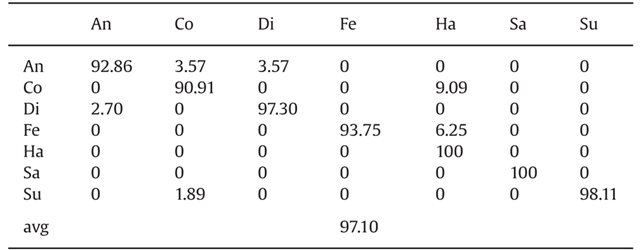
\includegraphics[width=0.7\linewidth]{images/15.png}
        \caption{Matrice di confusione del riconoscimento delle espressioni basato su Action Units usando Random Forest}
        \label{fig:image2}
    \end{center}
\end{figure}

Confrontando i risultati della Tabella riportata nell’immagine \ref{fig:image3}, dove sono raffigurati i tassi di riconoscimento della rete bayesiana, le prestazioni migliorano significativamente. 
\begin{figure}
    \begin{center}    
        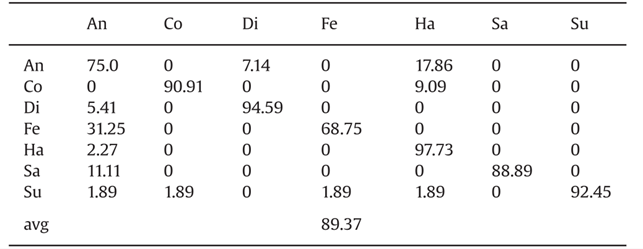
\includegraphics[width=0.7\linewidth]{images/16.png}
        \caption{Matrice di confusione del riconoscimento delle espressioni basato su Action Units usando Rete Bayesiana}
        \label{fig:image3}
    \end{center}
\end{figure}

Il classificatore con rete bayesiana ha un tasso di riconoscimento basso per le emozioni di tristezza e paura (rispettivamente 68,75\% e 88,89\%), mentre il random forest migliora queste prestazioni al 93,75\% e al 100\%.

Una possibile spiegazione è che la tristezza e la paura sono di solito poco evidenti e possono essere facilmente confuse con altre emozioni; tuttavia, il random forest ha maggiore capacità discriminativa e può trovare la differenza fra queste. 

Per giunta, i tassi di successo di emozioni come la rabbia, la sorpresa e il disgusto sono stati significativamente migliorati sfruttando il framework proposto. 

Per confermare l'efficacia del metodo, sono stati selezionati casualmente un set di training ed un set di testing dal dataset, per poi ripetere l'esperimento nove volte. Tutti i risultati sono riportati qui di seguito nell'immagine \ref{fig:image4}. 
\begin{figure}
    \begin{center}    
        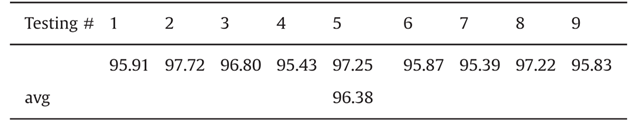
\includegraphics[width=1\linewidth]{images/17.png}
        \caption{Tasso di riconoscimento in percentule per le nove selezioni randomiche del training e test set}
        \label{fig:image4}
    \end{center}
\end{figure}

È stato dimostrato che il sistema ha una prestazione stabile utilizzando set di training e testing diversi. 
Il tasso di riconoscimento medio è significativamente più alto del metodo di confronto \cite{LearnExpresSpatTempManiFoldDynamFaceExpressReco}.

Un altro studio utilizzato per la predizione delle emozioni attraverso l’analisi delle Action Units è \cite{InferEmoFaceAUs}.
In questo studio viene proposto un metodo per mappare le AUs a sei emozioni:
\begin{itemize}
    \item anger,
    \item fear,
    \item happy,
    \item sad,
    \item surprise,
    \item disgust
\end{itemize}

Vengono selezionate delle Action Units, successivamente mappate alle emozioni attraverso relazioni statistiche e tecniche di matching.

Le relazioni fra le emozioni e le AUs sono collezionate come stringhe template che comprendono quelle più descrittive per ognuna delle emozioni trattate.

Le stringhe di template vengono poi computate usando un concetto chiamato discriminative power:

l’LCS, un metodo per approssimare il grado di coincidenza delle sottostringhe alla stringa di template, con l’applicazione del calcolo della prossimità fra le stringhe di test e la stringa di template della singola emozione.

Lo studio ha trovato che LCS è un metodo efficiente nella gestione di particolari problemi come il rilevamento errato delle AUs e aiuta a ridurre le predizioni false.

Il metodo proposto è stato testato su vari datasets:
\begin{itemize}
    \item CK+,
    \item ISL,
    \item FACS,
    \item JAFFE,
    \item Mind Reading,
    \item altri frame ripresi in condizioni in-the-wild
\end{itemize}

è stata poi effettuata una comparazione fra il metodo proposto e altri precedentemente presentati e si sono notati dei miglioramenti, sia sui datasets di benchmark che per quelli in-the-wild.\newpage

La procedura proposta basa il rilevamento delle AUs sul metodo offerto da \cite{RecoFaceExprMachLearnAppSpontBehav} e a seguire le Action Units vengono mappate con il metodo indicato nel paper, ed è visibile nell'immagine \ref{fig:image33}.
\begin{figure}
    \begin{center}    
        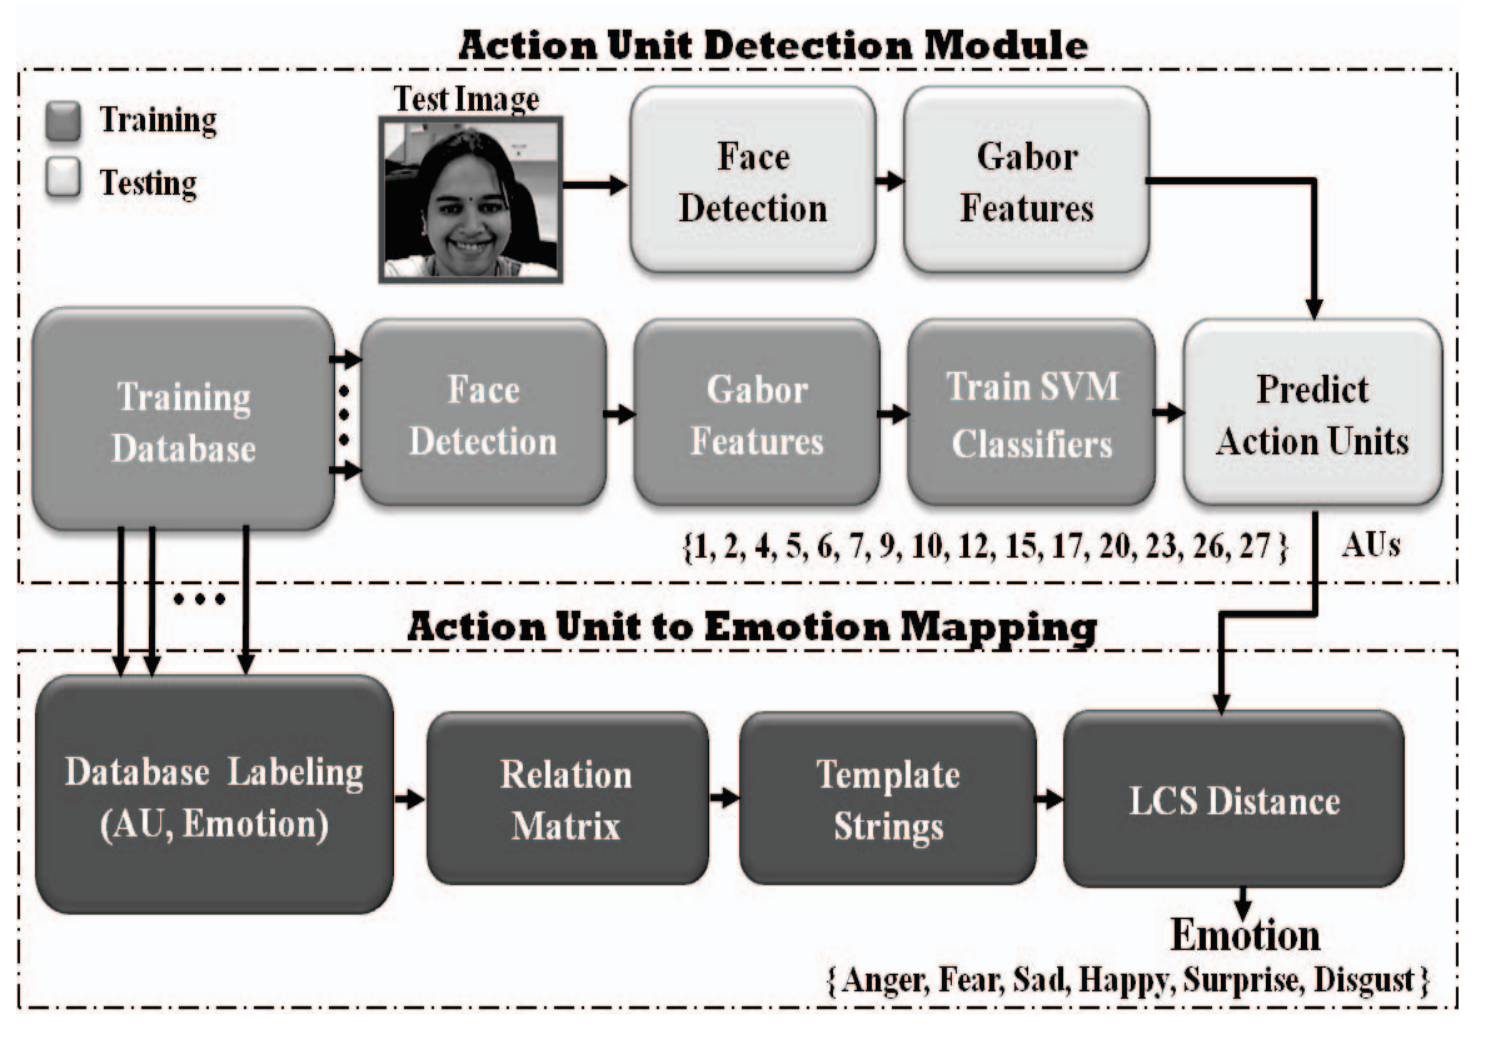
\includegraphics[width=0.7\linewidth]{images/18.png}
        \caption{Metodo di mappatura delle Action Units di \cite{RecoFaceExprMachLearnAppSpontBehav}}
        \label{fig:image33}
    \end{center}
\end{figure}

Per l’allenamento del modello volto al riconoscimento delle AUs sono state utilizzate 580 immagini dal CK+ dataset, e, per ognuna di queste, sono state effettuate varie modifiche alle immagini in modo da renderle adatte all’impiego; è stato applicato l’AdaBoost per la selezione delle feature al fine di ridurre la dimensione del vettore delle features, ed è stato utilizzato il Support Vector Machines (SVM) per il modello delle AUs.

Dopo un’attenta analisi del sistema FACS sono state scelte dai ricercatori quindici AUs, sufficienti per la rappresentazione delle sei emozioni che si sono proposti di identificare.

Le AUs rilevate vengono poi processate attraverso il modulo di mappatura per predire lo stato d’animo combaciante.

L’idea sulla quale il modello sviluppato in questo paper si fonda è che diversi metodi utilizzati per la rilevazione delle emozioni si basano su input (AUs) inaffidabili, in quanto sono presenti inevitabili errori nella localizzazione dei volti all’interno delle immagini.

È per questo che il loro metodo si concentra maggiormente sul trovare la correlazione fra le singole AUs e le emozioni che sulla diretta predizione di queste.

La relazione fra le Action Units e le sei emozioni si ottiene mediante un'analisi statistica del dataset di riferimento (CK+), etichettato sia per le emozioni che per le AUs. Le relazioni vengono acquisite sotto forma di una matrice relazionale derivata utilizzando un concetto chiamato discriminative power \cite{AutoInfereComplMentStatesVid}. 

Il discriminative power è definito come:
\[
H = P(Y_j|X_i) - P(Y_j|\overline{X_i})
\]
dove P(Yj |Xi) è la probabilità dell'azione $Yj$, dopo che $Xi$ è avvenuta, e $P(Yj | \overline{H_i})$ è la probabilità dell'azione $Yj$, dopo che l'emozione $H_i$ non è avvenuta. La dimensione di H rappresenta il potere discriminante di un'AU rispetto ad un'emozione.

La matrice relazionale viene ottenuta normalizzando H su tutte le AU per ciascuna delle emozioni. Pertanto, si ottengono pesi di associazione non lineari per ciascuna delle Action Unit, in base alla loro rilevanza per le emozioni calcolate servendosi dell'equazione sopra riportata.

La figura \ref{fig:image5} riporta la matrice di relazione calcolata per le sei emozioni. Qui, i valori positivi, rappresentati in bianco, indicano l'alta probabilità per un'AU di appartenere ad un'emozione; d’altra parte, i valori negativi, rappresentati in nero, indicano l'alta probabilità per un'AU di non essere associata ad un'emozione. 

Ad esempio, l'emozione happy è associata positivamente alle AU6, AU7, AU12, AU26 e negativamente alle AU1, AU2, AU5, AU9. 

I risultati sperimentali presentati dallo studio dimostrano che la matrice di relazione derivata è efficiente nell'identificazione delle azioni facciali altamente rilevanti e i loro pesi di associazione per le varie emozioni, e può quindi prevedere correttamente le emozioni.
\begin{figure}
    \begin{center}    
        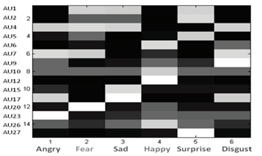
\includegraphics[width=0.6\linewidth]{images/19.png}
        \caption{Matrice di relazione calcolata sulle sei emozioni}
        \label{fig:image5}
    \end{center}
\end{figure}

Per ciascuna emozione sono state selezionate le prime N entrate da AU altamente discriminanti e queste sono state salvate come stringhe di template per i futuri abbinamenti delle Action Units. 

La lunghezza delle stringhe di template utilizzata è di cinque per gli esperimenti condotti dai ricercatori dello studio.\newpage
\begin{figure}
    \begin{center}    
        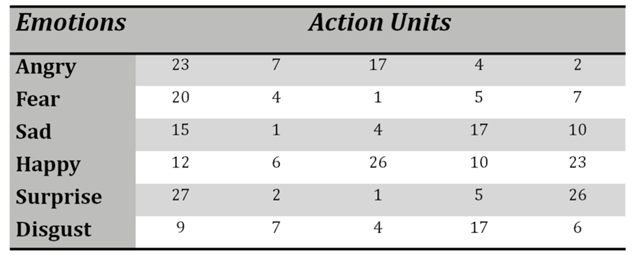
\includegraphics[width=1\linewidth]{images/20.png}
        \caption{Esempio di stringa template}
    \end{center}
\end{figure}

Date le stringhe con le Action Units per le immagini analizzate, queste vengono confrontate con le stringhe di template per trovare l'emozione corrispondente. 

Si utilizza la sotto sequenza comune più lunga (LCS) \cite{IntroToAlgo} per misurare la similarità tra le stringhe. LCS è un metodo per trovare la sotto sequenza più lunga fra tutte le sequenze date. 

In questo caso, una sotto sequenza è definita come una sequenza in cui le unità appaiono nello stesso ordine una rispetto all’altra, ma non necessariamente in modo contiguo. 

Ad esempio, nella stringa “ACTTGCG”, “ACT”, “ATTC” e “ACTTGC” sono tutte sotto sequenze. 

LCS permette "inserzioni", "eliminazioni" e "sostituzioni" delle singole AUs tra le stringhe. Questa caratteristica di LCS si è rivelata idonea per la predizione delle emozioni da stringhe di Action Units.

Per fare un esempio, data un'immagine di test, possono essere predette le combinazioni di AUs riportate nell’immagine \ref{fig:image6}.

In questo caso, la proprietà di eliminazione diventa importante per la mappatura delle diverse stringhe di Action Units come {AU12} o {AU6, AU12} o {AU6, AU12, AU26} all'emozione happy, poiché tutte indicano l’emozione di felicità pur mancando, alcune delle AU, nelle stringhe. 

Allo stesso modo, l'inserzione ha un ruolo nell’eliminazione delle AU rilevate erroneamente, come {AU1, AU4}, che comunque mappano l'emozione nella figura alla stringa di template che rappresenta l’emozione happy. 

Inoltre, permettere le sostituzioni aiuta a correggere gli errori di rilevazione che coinvolgono AU visivamente simili come AU12, AU20, AU23, e a predire l'emozione con un alto valore di confidenza. 

Viene evitata anche la mappatura errata di molte emozioni quando la stringa di test presenta errori considerevoli.
\begin{figure}
    \begin{center}    
        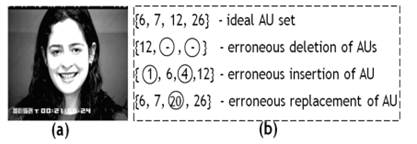
\includegraphics[width=1\linewidth]{images/21.png}
        \caption{Esempio di rilevamento delle Action Units}
        \label{fig:image6}
    \end{center}
\end{figure}

Ad esempio, in sostituzioni non condizionali, una stringa di test come 

\{{\colorbox{yellow}{AU4}, \colorbox{green}{AU6}, \colorbox{blue}{AU12}, \colorbox{cyan}{AU17}, \colorbox{magenta}{AU23}\}}, può essere mappata a 

\{{\colorbox{red}{AU1}, \colorbox{yellow}{AU4}, \colorbox{red}{AU10}, \colorbox{red}{AU15}, \colorbox{cyan}{AU17}\}} (tristezza) e 

\{{\colorbox{yellow}{AU4}, \colorbox{red}{AU6}, \colorbox{red}{AU7}, \colorbox{red}{AU9}, \colorbox{cyan}{AU17}\}} (disgusto) 

con un costo di sostituzione di "3". 

I risultati e l’accuratezza ottenuta dal metodo proposto dallo studio sui vari dataset utilizzati per valutarlo sono esposti nella tabella all'immagine \ref{fig:image7}:

\begin{figure}
    \begin{center}    
        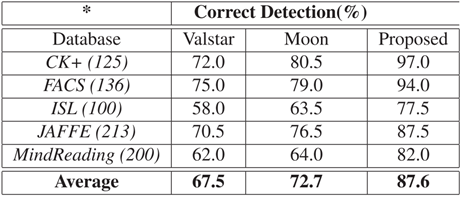
\includegraphics[width=1\linewidth]{images/22.png}
        \caption{Accuracy del metodo}
        \label{fig:image7}
    \end{center}
\end{figure}

\newpage

Analizzando altri papers sul soggetto, nessuno di questi mi è apparso particolarmente rilevante, in quanto carenti di metodologie che aggiungevano informazioni e metodi utili da unire ai lavori già ritrovati; inoltre i risultati di accuratezza e precisione ottenuti da questi sono inferiori rispetto agli studi già analizzati o insufficientemente migliori e necessitano di più risorse (tempo, quantità di dati e potere computazionale).

Ad esempio, in \cite{FaceEmoPredAUsDeepLearn} vengono confrontate le due principali tecniche di previsione delle emozioni facciali, ovvero le tecniche di apprendimento automatico (ML) e di deep learning (DL), in termini di accuratezza e livello di accountability. 
\begin{figure}
    \begin{center}    
        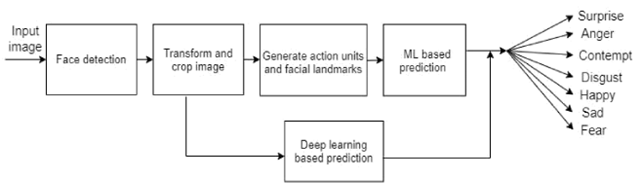
\includegraphics[width=1\linewidth]{images/23.png}
        \caption{Entrambi i process flow del riconoscimento delle emozioni facciali in \cite{FaceEmoPredAUsDeepLearn}}
    \end{center}
\end{figure}

Analizzando le due tecniche, i ricercatori hanno dimostrato che i modelli ML possono raggiungere risultati comparabili rispetto ai modelli DL. 

Nonostante la maggior parte delle ricerche recenti si siano focalizzate sulla costruzione di tecniche di Deep Learning per la predizione delle emozioni, si è scoperto che i modelli DL raggiungono prestazioni migliori a fronte di un costo elevato in termini di potenza di calcolo, di set di dati più grandi e di tempi di elaborazione più lunghi. 

Negli esperimenti sono stati conseguiti livelli di accuratezza del 86,66\% e dell'80\% rispettivamente per gli approcci DL e ML in termini di previsione delle emozioni; nonostante ciò, le tecniche di DL necessitano del supporto di una GPU ad alte prestazioni, mentre le tecniche ML possono ricoprire il proprio ruolo più velocemente anche senza il supporto di una GPU. 

Il beneficio più importante nell'utilizzo delle tecniche ML con le Action Units è la capacità di questi ultimi di poter giustificare l'emozione prevista in termini di contributo di ciascuna AU. 


\section{Studi che trattano campioni prelevati in scenari non controllati per una migliore precisione del modello}

Un altro problema trattato solo da \cite{PredLocStudEngagInTheWild} (fra i paper ritrovati a tema engagement e stati d’animo) e che invece ho notato più prominente all’interno della ricerca riguardo le emozioni FACS, è quello dei campioni denominati come “in-the-wild”.

Molti degli studi effettuati si concentrano su campioni prodotti in ambienti controllati, con nessun tipo di interferenza per quanto concerne i problemi che abitualmente si possono riscontrare quando invece si lavora con riprese che potrebbero avere una valenza anche quando le migliori condizioni non si presentano.

Come riporta \cite{AFEWVAdatabaseInTheWild}: “The videos are recorded under controlled conditions, e.g. illumination is uniform, background is static, and there is a limited amount of head pose variation and occlusion. Although a range of affective states are displayed and recorded, emotions are elicited by a limited number of tasks, e.g., in \cite{BelfastInducedNaturalEmotionDatabase}, all subjects underwent exactly the same tasks.”

Quindi i video creati in condizioni verificate, di luce uniforme, sfondo statico, con insufficienti variazioni nella posa delle persone, poca occlusione e dove le persone svolgono lo stesso compito non sono validi per creare un modello che possa effettuare delle predizioni veritiere da applicare ad ogni ambiente.

Per quanto riguarda la raccolta di immagini, negli studi “in the wild” è stato messo in atto il prelievo e la categorizzazione delle immagini da film, serie tv, e altri media che non rispettano gli standard imposti durante la creazione dei dataset prelevati invece in ambienti controllati \cite{AFEWVAdatabaseInTheWild}.

Per l’annotazione delle immagini sono stati consultati due annotatori esperti FACS AU che hanno individuato lo stato d’animo della/e persone presenti all’interno della scena presentata attraverso una piattaforma di tagging delle immagini.

Entrambi gli annotatori erano sempre presenti durante l’analisi dei singoli campioni ed hanno quindi potuto discutere ognuno dei casi incerti insieme; una volta concluse le prime analisi, sono stati inoltre ripresentati alcuni dei frame già analizzati agli stessi annotatori in modo da effettuare un’ulteriore verifica della loro consistenza, ed essi hanno dato la stessa annotazione l’87\% delle volte.

Per costruire il modello hanno poi utilizzato l’estrazione delle AU attraverso un sistema semi automatico, ed hanno utilizzato questi dati estratti per la costruzione del modello.

I risultati di queste analisi hanno portato alla conclusione che i modelli sviluppati attraverso raccolte di immagini prelevate in scenari controllati non portano necessariamente a risultati puntuali (o accurati) quando vengono applicati al mondo reale.
Una volta analizzati i sistemi utilizzati per l’elaborazione dei dati raccolti dai ricercatori che hanno redatto gli studi riportati precedentemente, ritengo ora necessario illustrare gli strumenti di cui si sono avvalsi.

\section{Metodologie di tagging delle immagini del dataset}
Per quanto riguarda la classificazione delle immagini dei dataset, vari studi hanno fatto ricorso a tecniche diverse:
\begin{itemize}
    \item Self report sul proprio stato emotivo da parte delle persone da cui vengono prelevati i campioni per le analisi, attraverso questionari o in modo arbitrario
    \item Valutazione da parte di esperti, spesso più di uno, per assegnare uno stato emotivo alle singole immagini o video; o scelto in modo interamente arbitrario da parte del/dei valutatore/i o utilizzando come riferimento lo stato emotivo riportato dalla persona
    \item Classificazione attraverso metodi di clustering \cite{FacialExpresRecLocalBinaryPatt}
\end{itemize}

Strumenti utilizzati per effettuare la classificazione:
\begin{itemize}
    \item Questionari a cui sottoporre i soggetti che vengono ripresi per la creazione del dataset
        \item \mbox{}\\[-\baselineskip]
        \begin{minipage}[t]{0.6\textwidth}
            In \cite{DAiSEE} è stata adoperata una tecnica di crowdsourcing: mediante la piattaforma Amazon Mechanical Turk (o MTurk) i ricercatori hanno specificato il task che si erano proposti di risolvere e hanno fornito i frame da analizzare. Questi sono stati poi suddivisi dalla piattaforma e categorizzati dai singoli individui (tale servizio è ovviamente retribuito)
        \end{minipage}\hfill
        \begin{minipage}[t]{0.3\textwidth}
            \centering
            \vspace{0pt}
            
\includegraphics[width=\textwidth]{images/12.png}
        \end{minipage}
\end{itemize}


\section{Estrazione delle feature facciali dalle immagini e dai video dei dataset}
Per quanto concerne l’estrazione dei dati dalle immagini, i paper analizzati hanno adoperato diverse librerie e strumenti fra cui:
\begin{itemize}
    \item OpenCV: libreria open-source di computer vision di cui ci si può avvalere per il riconoscimento delle espressioni facciali. OpenCV contiene diverse funzioni per l'estrazione delle AUs, come la rilevazione delle linee facciali e la stima dei parametri di deformazione.
    \item dlib: libreria di machine learning open-source che somministra funzioni per la rilevazione e l'analisi dei volti nelle immagini. Dlib è in grado di rilevare le AUs attraverso l'utilizzo di una rete neurale convoluzionale (CNN) addestrata su un grande dataset di espressioni facciali.
    \item FaceReader: software commerciale sviluppato dalla società olandese Noldus Information Technology che ricorre ad algoritmi di analisi dell'emozione per registrare e classificare le AUs nelle immagini facciali. FaceReader è capace di riscontrare fino a 20 AUs e di classificarle in base alle emozioni ad essi associate.
    \item OpenFace: framework open-source di computer vision sviluppato dall'Università di Carnegie Mellon che offre funzioni per l'estrazione delle AUs e la rilevazione delle espressioni facciali. OpenFace sfrutta una combinazione di tecniche di machine learning e di analisi geometrica per rilevare le AUs.
    \item FACET: software commerciale sviluppato dalla società americana Emotient che impiega una combinazione di tecniche di computer vision e di analisi dell'emozione per rilevare e classificare le AUs nelle immagini facciali. FACET è in grado di rilevare fino a 20 AUs e di classificarle in base alle emozioni associate.
    \item DeepFaceLab: software open-source che utilizza le deep neural networks per l'analisi dell'immagine e la manipolazione dei lineamenti. Può essere strumentalizzato per l'estrazione delle AUs da immagini facciali. 
    \item Per il progetto di tesi ho invece deciso di utilizzare:
    Pyfeat: libreria open-source sviluppata in Python per l’estrazione delle feature
    facciali dalle immagini. Pyfeat si basa sulla fruizione di un insieme di funzioni
    matematiche, dette funzioni di base, per descrivere la forma e l’aspetto delle suddette
    espressioni
\end{itemize}

Dopo aver analizzato i sistemi impiegati per l’elaborazione delle informazioni
ottenute dalle immagini ed aver illustrato il processo di estrapolazione di questi
dati, reputo possibile la creazione di un dataset ricavato dall’unione di alcuni dei
datasets citati precedentemente per lo studio di questa tesi.

\begin{figure}
    \begin{center}    
        
\includegraphics[width=0.3\linewidth]{images/pyfeat_logo_small.png}
        \caption{Logo py-feat}
    \end{center}
\end{figure}

\section{Unione dei dataset ritrovati e relativa categorizzazione delle immagini all’interno di questo}

I dataset utili ritrovati sono il DAiSEE \cite{DAiSEE} e il Student-engagement-dataset \cite{StudEngagDataset}.

\begin{itemize}
    \item DAiSEE presenta i seguenti mood:
    \begin{itemize}
        \item Boredom
        \item Engagement
        \item Confusion
        \item Frustration
    \end{itemize}
    \item Tutte con valore compreso fra 0 e 3:
    \begin{itemize}
        \item Inizialmente è stato chiesto ai labelers di annotare i frame a loro presentati con uno di questi tre tag:
        \begin{itemize}
            \item Looking at their paper
            \item Looking at their screen
            \item Wandering
        \end{itemize}
            
        Ognuno dei frame è stato assegnato almeno a tre persone, la label “vincente”, o meglio più frequente, è stata poi attribuita ai singoli frame.

        Infine, in base ai risultati ottenuti attraverso questa categorizzazione, conseguita via crowdsourcing, è stato conferito un valore fra 0 (non corrispondente) e 3 (del tutto corrispondente) ad ognuna delle classi precedentemente elencate.
    \end{itemize}
    \item Student engagement dataset, invece, presenta i seguenti mood:
    \begin{itemize}
        \item Confused (macro categoria: engaged)
        \item Engaged (macro categoria: engaged)
        \item Frustrated (macro categoria: engaged)
        \item Bored (macro categoria: not engaged)
        \item Drowsy (macro categoria: not engaged)
        \item Looking away (macro categoria: not engaged)
    \end{itemize}
\end{itemize}

Per la realizzazione del mio dataset ho ritenuto giusto attenermi alle classi proposte dallo Student Engagement dataset, in quanto propone più labels di cui usufruire.

Per mettere in atto ciò, è stato necessario unire i samples all’interno di DAiSEE ai samples dello student engagement dataset, per mezzo delle classi corrispondenti.

DAiSEE è provvisto di un maggior numero di samples, in quanto non solo racchiude molti più file, ma questi stessi sono video e non immagini, come nello student engagement dataset, naturalmente suddivisi in frame (2 immagini per ogni secondo di video).

Le classi che non trovano corrispondenza fra i due dataset (Drowsy e Looking away) potrebbero risultare meno frequenti e accurate nel riconoscimento; ho comunque preferito conservarle in quanto permettono una classificazione più ampia.

DAiSEE è un dataset realizzato tenendo in considerazione la questione “in-the-wild” e risulta quindi perfetto per lo studio proposto da questa tesi.

Lo student engagement dataset non è stato creato da una fonte autorevole e certificata come il DAiSEE ma, sfogliando le immagini presenti in esso, è possibile notare come gli scenari ripresi in questo dataset (ambienti di studio casalinghi) le immagini al suo interno risultino simili a quelle presentate nel DAiSEE e quindi della tipologia interessata.

\begin{table}[htb]
\small
\caption{estratto tabella AUs}
\label{Tab:Tabella_AUs}
\centering
    \begin{adjustbox}{angle=90}
        \begin{tabular}{|c|l|l|l|}
            \hline
            AU1 & Inner Brow Raiser & Frontalis (medial) & sadness, surprise, fear \\
            \hline
            AU2 & Outer Brow Raiser & Frontalis (lateral) & surprise, fear \\
            \hline
            AU4 & Brow Lowerer & Procerus, Depressor Supercilii, Corrugator Supercilii & sadness, fear, anger \\
            \hline
            AU5 & Upper Lid Raiser & Levator Palpebrae Superioris, Superior Tarsal Muscle & surprise, fear, anger \\
            \hline
            AU6 & Cheek Raiser & Orbicularis Oculi (orbital) & happiness, disgust, contempt \\
            \hline
            AU7 & Lid Tightener & Orbicularis Oculi (palpebral) & fear, anger \\
            \hline
            AU9 & Nose Wrinkler & Levator Labii Superioris Alaeque Nasi & disgust \\
            \hline
            AU10 & Upper Lip Raiser & Levator Labii Superioris & \\
            \hline
            AU11 & Nasolabial Deepener & Zygomaticus Minor & disgust, fear \\
            \hline
            AU12 & Lip Corner Puller & Zygomaticus Major & happiness, contempt \\
            \hline
            AU14 & Dimpler & Buccinator & contempt \\
            \hline
            AU15 & Lip Corner Depressor & Depressor Anguli Oris & sadness, disgust \\
            \hline
            AU17 & Chin Raiser & Mentalis & disgust \\
            \hline
            AU20 & Lip Stretcher & Risorius, Platysma & fear \\
            \hline
            AU23 & Lip Tightener & Orbicularis Oris & anger \\
            \hline
            AU24 & Lip Pressor & Orbicularis Oris & \\
            \hline
            AU25 & Lip Part & Depressor Labii Inferioris & happiness, surprise, fear \\
            \hline
            AU26 & Jaw Drop & Masseter, Temporalis, Medial Pterygoid & fear, surprise \\
            \hline
            AU28 & Lip Suck & Orbicularis Oris & \\
            \hline
            AU43 & Eyes Closed & Levator Palebrae Superioris (relaxation) & behavioral \\
            \hline
        \end{tabular}
    \end{adjustbox}
\end{table}
